\documentclass[conference]{IEEEtran}

% graphic declaration
\usepackage{graphicx}
\usepackage{listings}
\usepackage[english]{babel}
\usepackage{float}
\usepackage{color}
\usepackage{caption}
\usepackage{indentfirst}
\usepackage{amsmath}
\usepackage{fancybox}
\usepackage{algorithm}
\usepackage{algpseudocode}

\definecolor{dkgreen}{rgb}{0,0.6,0}
\definecolor{gray}{rgb}{0.5,0.5,0.5}
\definecolor{mauve}{rgb}{0.58,0,0.82}

\iffalse
\lstset{frame=tb,
  language=Java,
  aboveskip=3mm,
  belowskip=3mm,
  showstringspaces=false,
  columns=flexible,
  basicstyle={\footnotesize\ttfamily},
  numbers=none,
  numberstyle=\tiny\color{gray},
  keywordstyle=\color{blue},
  commentstyle=\color{dkgreen},
  stringstyle=\color{mauve},
  breaklines=true,
  breakatwhitespace=true,
  tabsize=3
}
\fi

\lstset{%
  numberstyle=\scriptsize\color[gray]{0.3},
  numbersep=5pt,
  stepnumber=1,
  numbers=left,
  xleftmargin=15pt,
  belowcaptionskip=\bigskipamount,
  captionpos=b,
  escapeinside={*'}{'*},
  language=Java,
  tabsize=2,
  emphstyle={\bf},
  commentstyle=\it,
  stringstyle=\mdseries\ttfamily,
  showspaces=false,
  keywordstyle=\bfseries,
  morekeywords={then,end},
  columns=flexible,
  basicstyle=\footnotesize\ttfamily,
  showstringspaces=false,
  morecomment=[l]\%,
}

\graphicspath{ {data/} }

\ifCLASSINFOpdf
  % \usepackage[pdftex]{graphicx}
  % declare the path(s) where your graphic files are
  % \graphicspath{{../pdf/}{../jpeg/}}
  % and their extensions so you won't have to specify these with
  % every instance of \includegraphics
  % \DeclareGraphicsExtensions{.pdf,.jpeg,.png}
\else
  % or other class option (dvipsone, dvipdf, if not using dvips). graphicx
  % will default to the driver specified in the system graphics.cfg if no
  % driver is specified.
  % \usepackage[dvips]{graphicx}
  % declare the path(s) where your graphic files are
  % \graphicspath{{../eps/}}
  % and their extensions so you won't have to specify these with
  % every instance of \includegraphics
  % \DeclareGraphicsExtensions{.eps}
\fi

% correct bad hyphenation here
\hyphenation{op-tical net-works semi-conduc-tor}


\begin{document}
%
% paper title
% Titles are generally capitalized except for words such as a, an, and, as,
% at, but, by, for, in, nor, of, on, or, the, to and up, which are usually
% not capitalized unless they are the first or last word of the title.
% Linebreaks \\ can be used within to get better formatting as desired.
% Do not put math or special symbols in the title.
\title{Job2P: Job Scheduling APIs for\\Wi-Fi Peer-to-peer Mobile Network}


% author names and affiliations
% use a multiple column layout for up to three different
% affiliations
\author{\IEEEauthorblockN{Le Dinh Minh}
\IEEEauthorblockA{Utah State University\\
minh.le@aggiemail.usu.edu}
\and
\IEEEauthorblockN{Young-Woo Kwon}
\IEEEauthorblockA{Utah State University\\
young.kwon@usu.edu}}


% make the title area
\maketitle

\begin{abstract}
These days, along with the rapid revolution of mobile device industry, software is also being built heavier and consumes more CPU performance and energy than they were in the past few years. Since the modern mobile devices support multiple connection methods like Wi-Fi, Bluetooth or NFC, the requirements of sharing the workloads and resources among the devices within a network to reduce full workload on an arbitrary device are being considered, especially in the areas Internet is not available, which can be found anywhere.

To address those limitations on mobile devices, we proposed Job2P as the Job Scheduling APIs for Android development that leverages Wi-Fi Direct to support sharing workloads and resources over peer-to-peer mobile device network, which doesn't require any Internet connections. Job2P provides a simple and straightforward API interface to get rid of sophistication of network implementation, letting developers easily create their distributed mobile applications with capability of forming closed range network. In term of workload distribution, Job2P splits task and resource into parts and packs them into the smaller units called jobs and dispatch to the peers. To distributed jobs equitably among the peers, a Decision Maker is added to decide the amount of resource the peer has to handle bases on its percentage of availability. Moreover, our APIs can handle fault tolerant for network malfunctions. 

Through our experiments with image processing, text processing and GPS location, we realized that Job2P improves significant productivity in term of performance and energy consumption. 
\end{abstract}


% For peer review papers, you can put extra information on the cover
% page as needed:
% \ifCLASSOPTIONpeerreview
% \begin{center} \bfseries EDICS Category: 3-BBND \end{center}
% \fi
%
% For peerreview papers, this IEEEtran command inserts a page break and
% creates the second title. It will be ignored for other modes.
\IEEEpeerreviewmaketitle



\section{Introduction}
These days, mobile phones have been playing a very important role in human society. People need their cellphone everyday for surfing Internet, searching for information, online shopping, communicating with friends, taking and sharing photos etc. As a result of highly intensive completions between the global mobile phone manufactures like Samsung and Apple, the cellphones are more and more equipped themselves with high specifications (CPU, RAM and built-in storage) and top functionality so that they are powerful enough in compare with those in the past or even with a desktop. 

With the hardware rapid development, software is also being built more and more sophisticated in many aspects. They may occupy more space on local storage, use more memory, and thus consume more energy. Even though the software is designed to run on mobile device, its size may vary up to 1GB (like image processing or image recognizing) and memory consumption can be up to 1GB as well. Since there are possibly many heavy workloads running on a device at some points, the needs of sharing workloads among the mobile devices is really necessary with respect to performance and energy efficiency. 

Distributed computing are so far well-developed in PC or embedded networks, bringing the synthesized power of computation from multiple computers to solve a problem. Up to now, there are thousands of solutions for the developers to create a distributed computing system. For instance, the emergency of a number of message-oriented middleware like DataTurbine \cite{rbnb}, RabbitMQ \cite{rabbitmq} or NaradaBrokering \cite{naradabrokering} lessened the effort of development for distributed applications to the minimum but still maintained all equipped functionality like data mirroring, dynamic network topology or fault tolerant. However, despite of stunning equipments, it is revealed that the most disadvantage of this kind of applications is the dependence of network connection or wireless access point. Without a network established, nothing happens.

Unlike the other PCs or wired devices, the mobile devices have their own advantage of multiple non-equivalent network capability. One of the remarkable network capability is installed on modern mobile devices are Wi-Fi Direct, which allows them to discover the others in any short distance less than 200 meters without utilizing Internet and wireless access point. No internet connections are required, and it will help the owner to connect to the devices within a closed distance. By establishing connection between the two devices to form a pair, Wi-Fi Direct can provide the simple way to dynamically initiate a peer-to-peer network. Available on Android devices from version 4.0 (which more than 96\% of devices are using these days), as well as a number of Intel-featured laptops and game consoles, there is the high possibility of discovering the other mobile devices at anywhere.

To address those limitations with heavy software on mobile devices, we proposed Job2P as the Job Scheduling APIs for Android development that leverages Wi-Fi Direct to support sharing workloads and resources over peer-to-peer mobile device network, which doesn't require any Internet connections. Job2P provides a simple and straightforward API interface to get rid of sophistication of network implementation, letting developers easily create their distributed mobile applications with capability of forming closed range network. In term of workload distribution, Job2P splits task and resource into the smaller units called jobs, and dispatch to the peers. To distributed jobs equitably among the peers, a decision making module is added to decide the amount of resource the peer has to handle bases on its percentage of availability. Moreover, our APIs can handle fault tolerant for network malfunctions.

Based on our experiments and results, our contributions are as follow
\begin{itemize}
	\item \textbf{Simple programming model} a library for developers facilitates establishing mobile peer-to-peer network.
	\item \textbf{Job Scheduler} for scheduling job execution and resource heterogeneity adaptation
	\item \textbf{Runtime system} determines the number of devices with according appropriate jobs for the remote execution bases on applied algorithm on level of availability.  
	\item \textbf{Systematic evaluation} our test case experiments will give the proof of APIs productivity
\end{itemize}
 

\section{Motivation and Technical Background}

\subsection{Motivation} %or {Motivating Examples}
\subsection{Technical Background}
\subsubsection{Machine-to-Machine Communication}
\subsubsection{Remote Execution}

\section{Proposed Approach: \emph{Job2P}}

\subsection{Approach Overview}
To retrieve the goals, as well as making our APIs widely adaptive to different context and usages, our consistent idea of design is hiding the complexity of system implementation and open to the developers the capability of customization. This below figure describes the internal architecture of a typical application utilizing our APIs to form a distributed mobile peer-to-peer system (Figure \ref{fig:architecture}). Basically, our system comprises of two main components:

\begin{figure}[H]
\centerline {
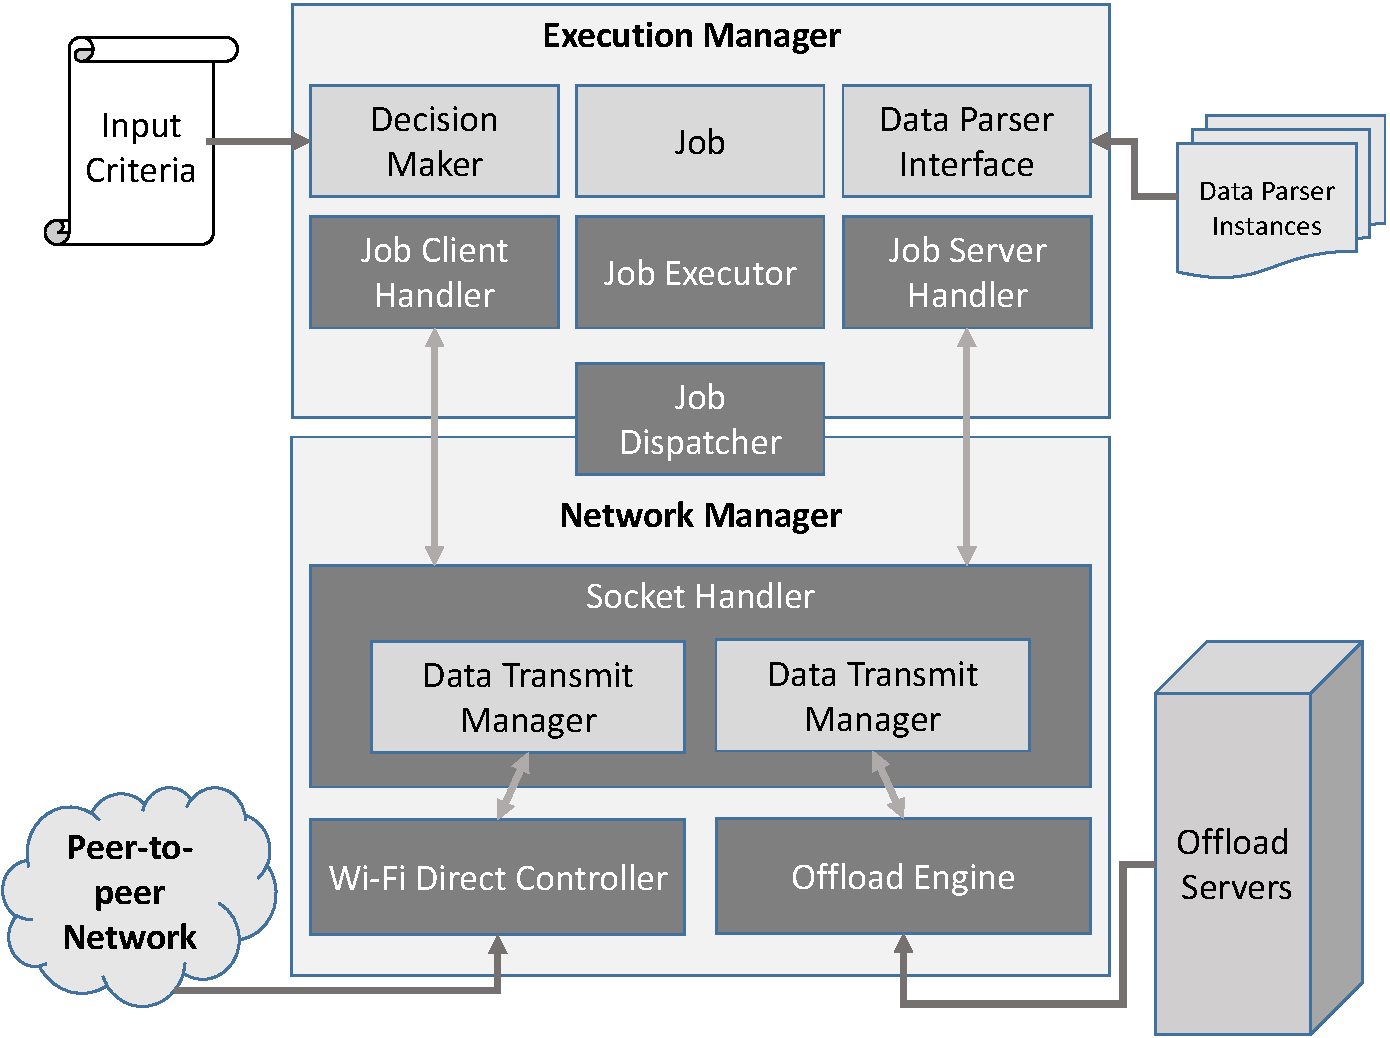
\includegraphics[width=0.39\textwidth, natwidth=643, natheight=559]{data/jobShareArch}
}
\caption{Job2P Architecture}
\label{fig:architecture}
\end{figure}

\begin{itemize}
	\item \textbf{Wi-Fi Peer-to-peer Broadcaster} (\texttt{WPB}) wraps up Wi-Fi Direct implementation, socket management and connection establishment. Moreover the \texttt{WiFiBroadcaster} provides a simplified API interface to form peer-to-peer network.
	\item \textbf{Job Handler} in charge of making decision on selecting available peers, determining and splitting the appropriate amount of jobs from the assigned task. The \texttt{JobDispatcher} sub module dispatches job and \texttt{JobExecutor} perform job execution at a single peer. Besides, \texttt{JobHandler} merges the scattered incoming results into the final placeholder and relay information messages to the main application.
\end{itemize}

\subsubsection{Wi-Fi Peer-to-peer Broadcaster}
To easily form up multiple pair connections between devices in the network, we utilized Wi-Fi Direct, the new feature available from Android APIs 4.0. We developed the \texttt{WiFiDirectManager} sub module inside the \texttt{WPB} to wrap up the complexity of Wi-Fi Direct implementation. Holding an instance of \texttt{WifiP2pManager}, \texttt{WiFiDirectManager} maintains connectivity over peer-to-peer network, discover available peers and setup the connections. 

When the app starts up, \texttt{WPB} from a peer will spread acknowledgments by calling \texttt{discoverPeers()} to inform its availability to the other peers. If a peer receives such message, its \texttt{WPB} module will collect information from the new comer and update the list of devices. When all the peers are updated with their new device list, the network will be reformed. See figure \ref{fig:forming}

\begin{figure}[H]
\centerline {
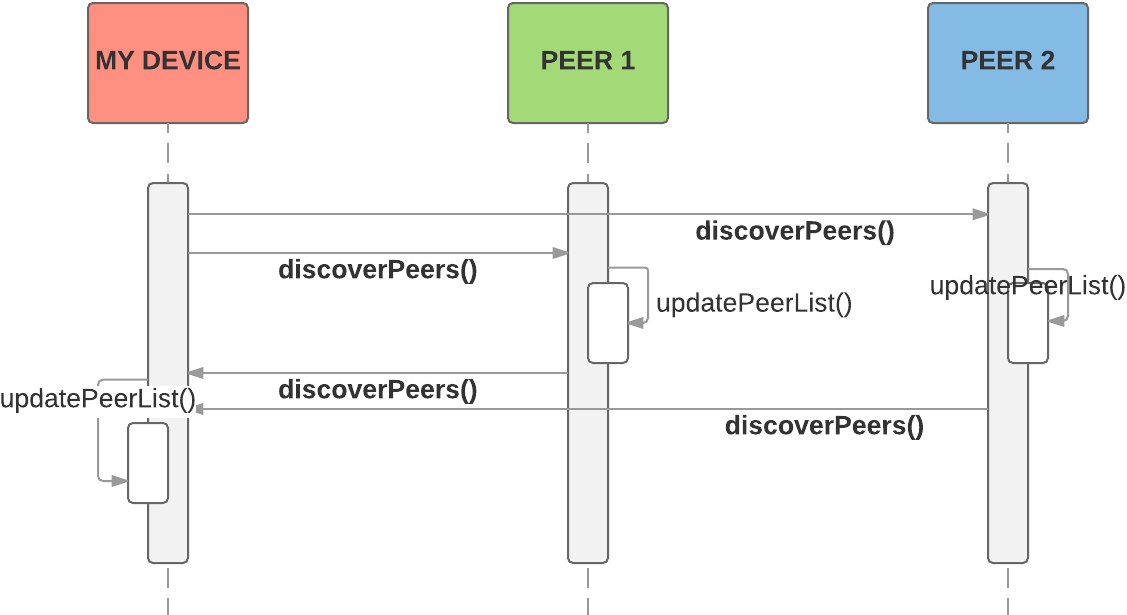
\includegraphics[width=0.5\textwidth, natwidth=1127, natheight=615]{data/discoverPeers}
}
\caption{Forming peer-to-peer network}
\label{fig:forming}
\end{figure}

When peers have information of the others, they are ready to connect. We provide function \texttt{connectToADevice()} holding \texttt{WifiP2pDevice} as one input parameter to invoke the handshake with another device. Once connection established, the device actively invoked will be assigned as client, which utilize the \texttt{ClientSocketHandler} to listen to a client socket. The device passively received the invocation will be promoted as server and use the \texttt{ServerSocketHandler} to initiate server socket with an random port. If the invoked device is already a server, it will maintain its current state and continuously accept the new client. Moreover, since a device can either be a server to some peers, or serve as client to the others, this method is able to build up a close range peer-to-peer network.

Both \texttt{ClientSocketHandler} and \texttt{ServerSocket Handler} are constituted by a sub module named \texttt{DataTransmitManager}, which periodically observes input and output streams of parent socket (Can be either server or client socket) to verify checksum, check data consistency, send/receive data from the socket. Inheriting the \texttt{TransmitManager} abstract class, developer can instantiate their own version of \texttt{DataTransmitManager} to customize the data consistency checker or improve security. 

\subsubsection{Job Handler}
\texttt{Job} is defined BLAH BLAH BLAH
\texttt{DataParser} is a loose coupling interface of the Job component facilitating adaptation with data heterogeneity. It helps determining mechanisms for: (1) serialization/deserialization object into binary format which is compatible for TCP transmission, (2) task partitioning, and (3) placeholder initialization and concatenation. To make the data type comprehensive to system in terms of reading, parsing or memory allocating, developer needs to supply instructions by instantiating an implementation of Data Parser for that type. 

\subsection{Programming Model of Job2P} 
\subsubsection{Job Definition}
To avoid any malfunctions and misconfiguration at remote execution, a conventional Job interface is defined like the code snipe below (\ref{code:job_def}) \\

\noindent \shadowbox{%
\begin{minipage}{239pt}
	\captionof{lstlisting}{Job Definition}
	\label{code:job_def}
	\begin{lstlisting}
	public class Job {
		public Object exec(Object partialObject) {
			// job implementation
		}
	}
	\end{lstlisting}
	
\end{minipage}}	

Where the body of \texttt{exec()} will contain concrete implementation of the Job.

Since Dalvik VM didn't support loading class the way Java VM does. Instead it will load Dalvik execution ("dex") files from an alternative locations such as internal storage or network. We provide \texttt{DexCreator} tool, the windows commandline application supports compiling the \texttt{Job} java file into the dex job package (a jar file). Dex package and sliced resources in binary format will be added into one \texttt{JobData} object by \texttt{JobDispatcher}, signed with checksum for consistency and dispatched to the other peers.

When client peer receives an object of \texttt{JobData} sent from server, it will firstly check checksum to confirm the consistency, then deserialize it into \texttt{Job} and resources and execute the job with that data.

\subsubsection{Data Parser}
The code snipe \ref{data_parser} shows the main functionality of the \texttt{DataParser} interface that user needs to comply. Under the first released version, we also support 3 basic Data Parsers for Image, Text and GPS.\\

\noindent \shadowbox{%
\begin{minipage}{245pt}
  \captionof{lstlisting}{\texttt{DataParser} interface}
  \label{data_parser}
  \begin{lstlisting}
public interface DataParser {
  ...
  
  public Class getDataClass();

  public byte[] parseObjectToBytes(dataObject);

  public Object parseBytesToObject(byteArray);

  public Object getSinglePart(..., numOfParts, 
										firstOffset, lastOffset);
    
  public Object createPlaceholder(jsonMetadata);

  public Object copyPartToPlaceholder(... 
									partDataObject, partIndex);

  public void destroy(dataObject);
  
}
  \end{lstlisting}	
\end{minipage}}	

To clarify usage of \texttt{DataParser}, we will go through several important abstract methods.

\begin{itemize}
	\item \texttt{getDataClass()} return data type.
	\item \texttt{parseObjectToBytes(object)} instructs system to serialize an object to binary array. In Android, not every object can be serialized, for instance Bitmap.  
	\item \texttt{parseBytesToObject(byte[])} deserialize a binary array back to object.
	\item \texttt{getSinglePart()} return a data slide bases on number of parts (\texttt{numOfParts}) and its \texttt{index}. Code snipe \ref{code:get_single_part} shows an example getting one slice from a bitmap by \texttt{index}. When app runs, \texttt{JobDispatcher} will use this method to partition the task into slices.
	\item \texttt{copyPartToPlaceholder()} Once partial result is retrieved from a distant peer, this function will instruct application to merge it to the placeholder.
\end{itemize}


\subsection{Job Scheduling and Decision Maker} \label{scheduling}

In peer-to-peer network supported by our APIs, the server will distribute jobs to peers bases on investigating their availability by \texttt{DecisionMaker} (Figure \ref{fig:checkStatus}). At the early stage before the transmission, the \texttt{DecisionMaker} of the calling device sends inquiring request for status (\texttt{IRS}) to some of selected peers in the network. If one receives this IRS request, its \texttt{DecisionMaker} will estimate its capability of response using the measurements of CPU, memory and battery usage at that time. 

\begin{figure}[H]
\centerline {
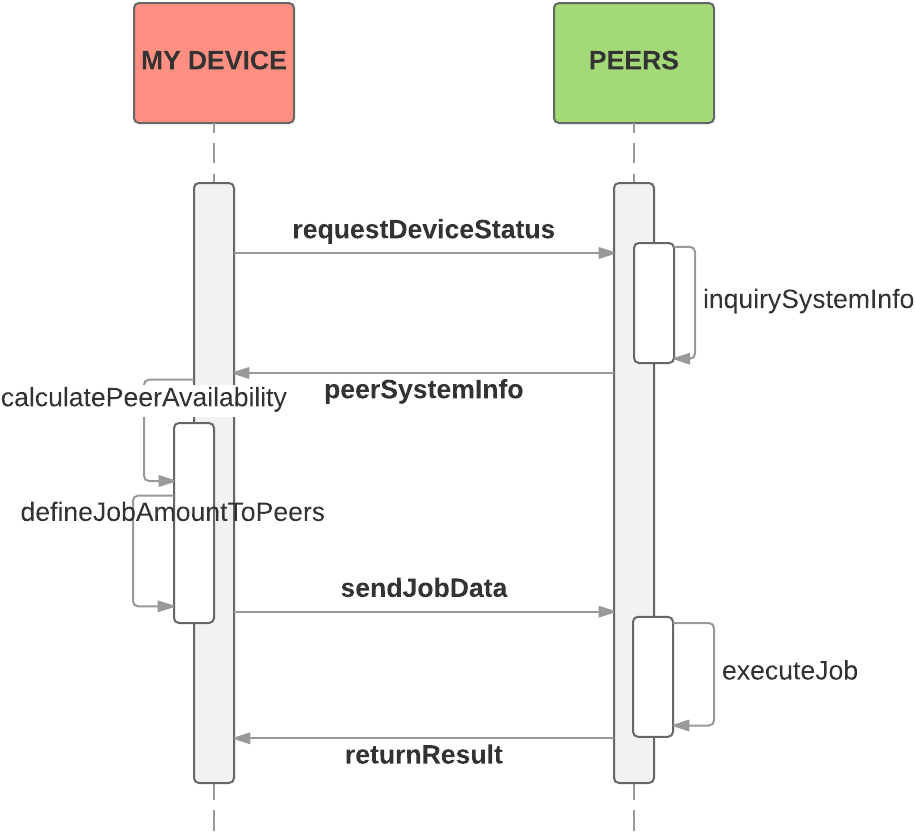
\includegraphics[width=0.45\textwidth, natwidth=915, natheight=837]{data/checkStatusFlow}
}
\caption{Decision making workflow}
\label{fig:checkStatus}
\end{figure}

\subsubsection{Detect feasible peers}\label{ss_dfp}

A mobile device at any time maintains a certain number of connection with the others. Before delivering jobs, it dispatches IRS messages to all the peers for acknowledgment of their availability ($RL$ - Level of Responsibility). If a peer receives an IRS, its \texttt{DecisionMaker} will capture its configuration and corresponding usage states to generate a response in JSON format, The code snipe \ref{code:jsonResponse} shows such a typical response.\\

\noindent \shadowbox{%
\begin{minipage}{239pt}
\captionof{lstlisting}{JSON response from peer}
\label{code:jsonResponse}
	
\begin{lstlisting}
{
  "device" : "LG-Volt",
	"RL" : 24.83,
  "availability" : "low",
	"network" : "low",
	"gps" : "on",
  "cpu" : {
		"usage" : "0.3",
    "speed" : "1.3",
    "cores" : 4
	},
  "memory" : {
		"usage" : "0.5",
    "total" : 2
  },
  "battery" : {
		"usage" : 0.85,
    "total" : 2800
  }
}
\end{lstlisting}
	
\end{minipage}}	

Where $RL$ is peer's Level of Responsibility (for estimation of $RL$ as well as the other usage parameters, see \ref{ss_jqfp}), \texttt{availability} indicates whether the peer is feasible for handling job. \texttt{network} gives the network status, which can be either \texttt{high}, \texttt{low} or \texttt{off} (no connections), \texttt{gps} is information of GPS \texttt{on} or \texttt{off}. Finally \texttt{cpu}, \texttt{memory} and \texttt{battery} are statuses of the essential resources at the time of response. 

In any IRS response, parameter \texttt{availability} can be assigned with value of \texttt{low}, \texttt{medium} or \texttt{high}. The \texttt{low} availability will inform the calling peer that it is not available due to temporary resource limitation, therefore eliminate the caller from sending jobs to. Only the peers with \texttt{availability} higher than \texttt{medium} will accept jobs for execution. The decision is given bases on the thresholds of battery usage which are set by default at value higher than 0.8 (or 80\% overall usage) for the \texttt{low}, 0.5 to 0.8 for the \texttt{medium} and lower than 0.5 for the \texttt{high}. User can override those thresholds by updating the \texttt{availability-thresholds} in the configuration file before app initialization. 

In the above example (code snipe \ref{code:jsonResponse}), the battery usage was 0.85 or 15\% remained, so the \texttt{DecisionMaker} on it stated that its \texttt{availability} is \texttt{low}, in other words it is not able to handle any jobs and should be excluded from the dispatched list.

\begin{algorithm}

\caption{Select Available Peers Algorithm}
\label{alg:select_peers}
\begin{algorithmic}[1] 
\begin{footnotesize}
\Function{selectPeers()}{}
\State Send IRS requests to all peers 
\State $P_{AV} \leftarrow HashMap(DeviceId, P)$
\ForAll{$Resp_{IRS}$ in \{Incoming IRS Responses\}}
\If {$Resp_{IRS}[availability] = low$} 
   \State continue;
\Else
  \State $P_{Info} \leftarrow P2pDevice[DeviceId] + Resp_{IRS}[RL]$
  \State $P_{AV}[DeviceId] \leftarrow P_{Info}$
\EndIf
\EndFor
\State \Return $P_{AV}$
\EndFunction
\end{footnotesize}
\end{algorithmic}

\end{algorithm}

The algorithm \ref{alg:select_peers} explains how the caller select the suitable peers from its connection list. Where $P_{AV}$ stands for map of available peers and $P2pDevice$ is the device information list.\\

\subsubsection{Job quantitation for peers}\label{ss_jqfp}

The calling peer quantitates the jobs from a task to distribute to the other available devices in the network suitably. To achieve this, the $RL$ parameter will be used as the main coefficient for the split. 
 
To calculate $RL$ as well as the other parameters in IRS, retrieved from \texttt{/proc/stat} system file \cite{stat_explain}, the percentage of CPU usage is expressed by this following expression in two short consecutive times

$$Usage_{CPU} = \frac{(\sum{T_{CPU2}} - T_{Idle2}) - (\sum{T_{CPU1}} - T_{Idle1})}{(\sum{T_{CPU2}} - \sum{T_{CPU1}})}$$

When $\sum{T_{CPU}}$ is total time of running CPU and $T_{Idle}$ is idle time correspondingly in hertz. In term of memory usage, the $Usage_{Mem}$ can be determined by using \texttt{MemoryInfo} from Android API to retrieve $Mem_{Avail}$ and $Mem_{Total}$, so the $Usage_{Battery}$.

Since in the mobile device, the lower resource usage state states the higher availability, and the higher specifications represents the better responsibility. Then the level of responsibility of device can be simply summarized by the below expression

$$RL = \frac{CPU_{Spec}}{Usage_{CPU}} + \frac{Mem_{Spec}}{Usage_{Mem}} + \frac{Battery_{Spec}}{Usage_{Battery \times 1000}}$$

Where $CPU_{Spec}$ has GHz unit, $Mem_{Spec}$ has GB unit and $Battery_{Spec}$ has uAh unit. Especially $CPU_{Spec}$ is determined by number of its core. For example, a quad-core CPU at speed of 1.3GHz can be counted as $1.3 \times 4$ or 5.2. At a certain time of that device, if $Usage_{CPU}$ is 0.3, $Usage_{Mem}$ is 0.5 (half of 1GB memory consumed), $Usage_{Battery}$ is 0.7 or 70\% used over a 2800uAh capacity battery, the value of $RL$ will be

$$RL = \frac{5.2}{0.3} + \frac{1}{0.5} + \frac{2800}{0.7 \times 1000} = 23.33$$

To reduce the latency and to avoid miscalculation at the calling peer, $RL$ is prematurely calculated by each available called peer and wrapped up in the IRS response sending back to the caller. 

In a peer-to-peer network comprising of $n$ devices, where $i$-device has responsibility level $RL_{i}$, the \texttt{DecisionMaker} will assign the job with carrying amount of data ($M_{i}$) which is equivalent to

$$M_{i} = M\frac{RL_{i}}{\sum_{j = \overline{1,n}}{RL_{j}}}$$

Where $M$ is total size of data in bytes. This below algorithm \ref{alg:assign_job} will represent the procedure that \texttt{DecisionMaker} judge the peer capability to assign the appropriate job. Where $M_{i}$ is quantity of job in binary length, $firstOffset$ and $lastOffset$ indicate the location of the data trunk in the whole.

\begin{algorithm}
\caption{Assign Job Algorithm}
\label{alg:assign_job}
\begin{algorithmic}[1]
\begin{footnotesize}
\Function{assignJobs()}{}
\State $M \leftarrow {getDataSize()}$
\State $RL_{Total} \leftarrow 0$ 
\For {$P$ in \{$P_{AV}$\}}
  \State $RL_{Total} \leftarrow RL_{Total} + P[RL]$
\EndFor
\\
\State $firstOffset, lastOffset \leftarrow 0$
\State $jobData \leftarrow Null$
\State $job \leftarrow {readJobFile()}$
\State $M_{C} \leftarrow 0$
\\
\For {$i = 1$ to $P_{AV}.length$}\\
  \State $M_{i} \leftarrow M\frac{RL_{i}}{RL_{Total}}$\\
  \State $firstOffset \leftarrow M_{C} $
  \State $lastOffset \leftarrow M_{C} + M_{i}$
  \State $jobData \leftarrow DataParser.getSinglePart($
  \State 
		\hspace{\algorithmicindent}
		\hspace{\algorithmicindent}
		\hspace{\algorithmicindent}
		\hspace{\algorithmicindent}
		\hspace{\algorithmicindent}
						$firstOffset, lastOffset)$
  \State $dispatchJob(\{job, jobData\})$\\
  \State $M_{C} \leftarrow lastOffset$
  
\EndFor

\EndFunction
\end{footnotesize}
\end{algorithmic}
\end{algorithm}

\subsection{Estimating Energy Consumption in WiFi Environment}
Assume that we have a Wi-Fi peer-to-peer network available with $n$ devices, each device at a certain time has level of responsibility $RL_{i} (i = \overline{1,n})$. According to the section \ref{scheduling}, if $E$ is the energy consumed by the application for only completing the task regardless of other ambiances, the total energy $E_{0}$ will be

$$E_{0} = E + E_{w}$$

Where $E_{w}$ is energy the app requires for waiting. Also, 

$$E_{p2p} = E(\frac{RL_{0}}{\sum_{i = 1}^{n}{RL_{i}}}) + E_{WiFi} + E_{w}$$ 

Where $E_{WiFi}$ is energy consumed by Wi-Fi for sending jobs to other peers.

In this estimation we skipped considering $E_{w}$ since it will depend on appearance of applications. If application have no GUI like system background services, $E_{w}$ will cause very little effect. From the two above equations, we can get the difference energy consumption between the two job processing mechanisms $E_{Diff}$ 

$$E_{Diff} = E_{0} - E_{p2p}$$ or $$E_{Diff} = E(1 - \frac{RL_{0}}{\sum_{i=1}^{n}{RL_{i}}}) - E_{WiFi}$$

According to \cite{wifi_energy}, Wi-Fi caused battery drained linearly by time during the transmission, particularly the drain can be represented by $y = 17.01x - 0.93$ for downloading and $y = 17.31x - 2.28$ for uploading. Therefore, it is inferred that in a mobile system with a certain number of devices in different levels of responsibility, if E is big enough, in other words, if the task to perform is big enough, then $E_{Diff} > 0$ will happen, thus deploying a peer-to-peer cluster will give the great benefit in term of energy efficiency. The bigger value of $E_{Diff}$, the more benefit we will archive.

\subsection{API Usage Scenario}

The library should be simple, so that developer can integrate within just a few steps. This section will describe step-by-step the way to utilize our API to enable a typical peer-to-peer network.

\subsubsection{Defining a Job}

Job implementation is the prerequisite work to determine what to execute on the remote device and how to cast and manipulate data from the abstract object. According to section \ref{job-description}, developer needs to implement the Job class file separately by overriding the \texttt{exec()} method and cast the input abstract parameter to the concrete. Then run the \texttt{DexCreator} tool on the Job class to compile and compact it into the DEX jar package. The final outcome is the \texttt{job.jar} file, it should be saved in the internal storage of the caller device. To simplify, we can store it in the \texttt{Download} folder.  

\subsubsection{Implementing an Application Using APIs}

This sub section will describe 3 basic steps to implement an Android application to utilize our APIs

\paragraph{Message Handler}

The Message Handler is required to instantiate at the beginning. In particular, an instance of \texttt{UIHandler} is initiated to receive messages from system when it goes into runtime. While system is in progress, the log and information messages will periodically be returned with label \texttt{MAIN\_INFO} (Snipe code \ref{ui_handler}). When each job result comes, \texttt{JobHandler} will collect and handle by  to partially put into a placeholder. When all results arrived, the placeholder with label \texttt{MAIN\_JOB\_DONE} will be returned to inform the completion of job collaboration, as well as bring the final result back to the main app UI.\\

\noindent \shadowbox{%
\begin{minipage}{239pt}
	\captionof{lstlisting}{UI handler}
    \label{ui_handler}
	\begin{lstlisting}
	Handler mainUiHandler = new Handler() {
		@Override
		public void handleMessage(Message msg) {
			switch (msg.what) {
				case Utils.MAIN_JOB_DONE: {
					// when job is completely finished
				}
				case Utils.MAIN_INFO: {
					// to receive messages from the processor
				}
			}
		}
	};
	\end{lstlisting}

\end{minipage}}

\paragraph{Data Parser}

Secondly, developer needs to declare \texttt{DataParser} to determine data-type and parser to equip for manipulating data at run-time (see sub section \ref{job-description}). \texttt{JobHandler} is the main component which wraps up the complexity , and exposes only the necessary functions like \texttt{discoverPeers()} and \texttt{dispatchJob()}. To send ACK messages to other peers for exchanging acknowledgments and reforming network, we need to call \texttt{discoverPeers()} function on the program, this work should be done as soon as application starts. 

\noindent \shadowbox{%
\begin{minipage}{245pt}
  \captionof{lstlisting}{Example of \texttt{getSinglePart()} for Bitmap}
  \label{code:get_single_part}
  \begin{lstlisting}
@Override
public Object getSinglePart(data, partNum, idx){
  Bitmap bmpData = (Bitmap) data;
  int pWidth = bmpData.getWidth() / partNum;
  return Bitmap.createBitmap(bmpData, 
                  (pWidth * idx), 0, pWidth, 
                  bmpData.getHeight());
}
  \end{lstlisting}	
\end{minipage}}	

\paragraph{Discovery Peer and Dispatching Jobs}

When network is formed and connections are held from some of the peers, \texttt{dispatchJob()} will be call to locate the resources and job which predefined in local storage, it then invokes \texttt{DecisionMaker} (sub section \ref{scheduling}) for job splitting and binary serialization. Finally jobs will be dispatched over the socket\\

\noindent \shadowbox{%
\begin{minipage}{245pt}
	\captionof{lstlisting}{Declare DataParser and JobHandler}

	\begin{lstlisting}
	// data parser: to determine datatype how to split the data 
	dataParser = new BitmapJobDataParser();
	...
	// handlers registration
	jobHandler = new JobHandler(this, dataParser);
	jobHandler.setSocketListener(
		new JobHandler.JobSocketListener() {
			@Override
			public void socketUpdated(... isConnected){
					// when socket is updated
			}
	});
	...
	// update the device list
	deviceList.setAdapter(
		jobHandler.getDeviceListAdapter());
	...
	// send ACK to other members to reconstruct network
	jobHandler.discoverPeers();
	...
	// address resources and job to execute
	String dataPath = downloadPath + "/mars.jpg";
  String jobPath = downloadPath + "/Job.jar";
  jobHandler.dispatchJob(dataPath, jobPath);

	\end{lstlisting}

\end{minipage}}

\section{Evaluation}

\subsection{Micro Benchmark}

\subsection{Case Study}
To measure the performance of the system equipped with our APIs, we decorated a small testbed with collaboration of 5 different Android devices to perform our 3 test cases:
\begin{itemize}
	\item \textbf{Image Processing} we will initiate the peer-to-peer network test to perform blurring a large scale image which is unable to process at any of our devices. Particularly, to process an image with size $4000 \times 4000$ and 4 bytes to express each pixel color, application must spare the amount of memory equivalent to 64MB which is too expensive for the system, occasionally this kind of image would be refused to load. 
	\item \textbf{Text analysis} another proof of performance on text processing. Our APIs will yield the data parser to developer for data heterogeneous adaptation.
	\item \textbf{GPS} establishing a GPS connection is proof of high energy consuming. It would be impossible for a device with low battery to keep update with GPS frequently. We will base on Job2P to build a simple system so that one device can benefit GPS locations from the healthier devices.
\end{itemize}

\subsection{Results}

\subsubsection{Performances}
Diagrams go here


\subsection{Discussion}


\section{Related Work}
\label{sec:related}

\section{Conclusions}
\label{sec:conc}
The conclusion goes here.




% conference papers do not normally have an appendix


% use section* for acknowledgment
\section*{Acknowledgment}


The authors would like to thank...





% trigger a \newpage just before the given reference
% number - used to balance the columns on the last page
% adjust value as needed - may need to be readjusted if
% the document is modified later
%\IEEEtriggeratref{8}
% The "triggered" command can be changed if desired:
%\IEEEtriggercmd{\enlargethispage{-5in}}

% references section

% can use a bibliography generated by BibTeX as a .bbl file
% BibTeX documentation can be easily obtained at:
% http://mirror.ctan.org/biblio/bibtex/contrib/doc/
% The IEEEtran BibTeX style support page is at:
% http://www.michaelshell.org/tex/ieeetran/bibtex/
%\bibliographystyle{IEEEtran}
% argument is your BibTeX string definitions and bibliography database(s)
%\bibliography{IEEEabrv,../bib/paper}
%
% <OR> manually copy in the resultant .bbl file
% set second argument of \begin to the number of references
% (used to reserve space for the reference number labels box)
\begin{thebibliography}{100}

\bibitem{rbnb}
Sameer Tilak, Paul Hubbard, Matt Miller, and Tony Fountain, \emph{The Ring Buffer Network Bus (RBNB) DataTurbine Streaming Data Middleware for Environmental Observing Systems}, p125-133, e-Science and Grid Computing, Bangalore 2007.

\bibitem{rabbitmq}
Maciej Rostanski, Krzysztof Grochla, Aleksander Seman, \emph{Evaluation of highly available and fault-tolerant
middleware clustered architectures using RabbitMQ}, p879-884, FedCSIS 2014.

\bibitem{naradabrokering}
Gadgil, H.; Fox, G.; Pallickara, S.; Pierce, M. \emph{Managing grid messaging middleware}, Challenges of Large Applications in Distributed Environments, p83-91, 2006 IEEE

\bibitem{classloader}
Fred Chung, \emph{Custom Class Loading in Dalvik}, http://android-developers.blogspot.com/2011/07/custom-class-loading-in-dalvik.html, July 2011

\bibitem{stat_explain}
\emph{/proc/stat Explained}, http://www.linuxhowtos.org/System/procstat.htm

\bibitem{wifi_energy}
Kalic, G., Bojic, I., Kusek, M., \emph{Energy consumption in android phones when using wireless communication technologies}, p754-759, MIPRO May 2012

\bibitem{live_video_collaboration}
Marco de Sa, David A. Shamma, Elizabeth F. Churchill, \emph{Live mobile collaboration for video production: design, guidelines, and requirements}, p693-707, Journal of Personal and Ubiquitous Computing, Volume 18 Issue 3, March 2014

\bibitem{coast}
Cong Shi, Kaustubh Joshi, Rajesh K. Panta, Mostafa H. Ammar, Ellen W. Zegura, \emph{CoAST: collaborative application-aware scheduling of last-mile cellular traffic}, p245-258, MobiSys 2014

\bibitem{rio}
Ardalan Amiri Sani, Kevin Boos, Min Hong Yun, and Lin Zhong, \emph{Rio: a system solution for sharing i/o between mobile systems}, p259-272, MobiSys 2014


\end{thebibliography}

\end{document}


